\documentclass[10pt]{article}
\usepackage[utf8]{inputenc}
\usepackage{empheq}
\usepackage[inline, shortlabels]{enumitem}
\usepackage{gensymb}
\usepackage{multicol}
\setlength{\parskip}{0.5cm plus4mm minus3mm}
\setlength{\parindent}{0pt}
\usepackage{amsmath}
\usepackage{upgreek}
\usepackage[nobreak=true]{mdframed}
\usepackage[shortlabels]{enumitem}
\usepackage[margin=0.8in]{geometry}
\usepackage{changepage}
\usepackage{amssymb}
\usepackage{tikz}
\usetikzlibrary{arrows}
\usepackage{titlesec}
\usepackage{chngcntr}
\usepackage{graphicx}
\newcommand{\norm}[1]{\lvert #1 \rvert}
\newcommand{\Est}[1]{\hat{#1}}
\newcommand{\argmax}{\operatornamewithlimits{argmax}}
% \vspace{-5ex}
\begin{document}
\date{}
\title{\vspace{-5ex}Final Cheat Sheet - EE16A Spring 2016\vspace{-5ex}}
\maketitle
\begin{multicols}{2}
\begin{enumerate}
    \item \textbf{Inner Products} \\
    The dot product of vectors $\vec{u}$ and $\vec{v}$ $\in$ $\mathbb{R}^n$ is defined as:
    \begin{equation*}
       \langle \vec{u} , \vec{v} \rangle = \vec{u}^T\vec{v} = \begin{bmatrix} u_1 & \hdots & u_n \end{bmatrix}
        \begin{bmatrix} v_1 \\ \vdots \\ v_n \end{bmatrix}
       = u_1v_1+\ldots u_nv_n
    \end{equation*}
    Properties:
    \begin{align*}
        \langle \vec{u} , \vec{v} \rangle  = \langle \vec{v} , \vec{u} \rangle \\
        \langle c\vec{u} , \vec{v} \rangle = c\langle \vec{u} , \vec{v} \rangle \\
        \langle \vec{u} +\vec{x}, \vec{v} \rangle = \langle \vec{u} , \vec{v} \rangle + \langle \vec{x} , \vec{v} \rangle
    \end{align*}
    The Euclidean norm (length) of a vector is defined as:
    \begin{equation*}
        \norm{\norm{\vec{u}}}=\sqrt{\langle \vec{u}, \vec{u} \rangle}
    \end{equation*}
    For vector lengths:
    \begin{equation*}
        \langle \vec{u}, \vec{v} \rangle=\norm{\norm{\vec{u}}}\hspace{.5mm}\norm{\norm{\vec{v}}}\cos{\theta}
    \end{equation*}
    Cauchy-Schwartz Inequality:
    \begin{align*}
        \norm{\langle\vec{x},\vec{y}\rangle} \leq  \norm{\norm{\vec{x}}} \cdot \norm{\norm{\vec{y}}}
    \end{align*}
    The projection of a vector $\vec{y}$ onto another vector $\vec{x}$ is given by:
    \begin{align*}
        \Est{y} = \frac{\langle \vec{y} , \vec{x} \rangle}{\langle \vec{x} , \vec{x} \rangle}\vec{x}
    \end{align*}
    Similarly, the projection of a vector $\vec{y}$ onto a subspace $W$ is given by
    \begin{align*}
        \Est{y} = \frac{\langle \vec{y} , \vec{u_1} \rangle}{\langle \vec{u_1} , \vec{u_1} \rangle}\vec{u_1}
        + \hdots + \frac{\langle \vec{y} , \vec{u_n} \rangle}{\langle \vec{u_n} , \vec{u_1} \rangle}\vec{u_n}
    \end{align*}
    where $\left\{\vec{u_1}, \hdots, \vec{u_n}\right\}$ form an orthogonal basis for $W$. 
    \item \textbf{Correlations} We use inner products as a similarity measure between vectors in the context of
    searching for a time-shift of a beacon signal. We cross-correlate a signal $\vec{s_1}$ and signal $\vec{s_2}$ by first constructing the circulant matrix $C_{\vec{s_1}}$ of $\vec{s_1}$ (an $N$ x $N$ matrix whose $i^{th}$ column is the $i^{th}$ rotation of $\vec{s_1}$; this matrix should be approximatelty orthogonal). Then the cross-correlation of $\vec{s_2}$ with all shifts of $\vec{s_1}$ is $C_{\vec{s_1}}^T\vec{s_2}$. The index of the maximum of the plot of this vector represents the time-delay of the signal. Autocorrelation is cross-correlating a vector with itself.
    
    \item \textbf{Triangulation} After finding the time-delays of signals, we can find the distances to each beacon based on knowing the speed of the wave. Assuming we know the locations of the beacons, we can now find our position. 
    \begin{align*}
        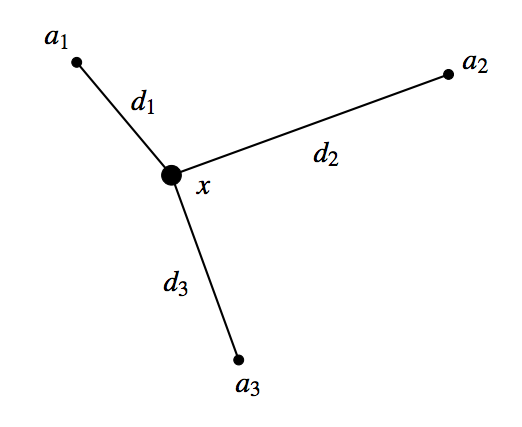
\includegraphics[scale=0.25]{loc.png}
    \end{align*}
    Using some tricks to make the terms linear, we can solve for $\vec{x}$ with
    \begin{align*}
        \begin{bmatrix} 
        2 \left( \vec{a_1}-\vec{a_2} \right)^T \\
        2 \left( \vec{a_1}-\vec{a_3} \right)^T 
        \end{bmatrix}
        \vec{x} = 
        \begin{bmatrix}
        \norm{\norm{\vec{a_1}}}^2-\norm{\norm{\vec{a_2}}}^2-d_1^2+d_2^2 \\
        \norm{\norm{\vec{a_1}}}^2-\norm{\norm{\vec{a_3}}}^2-d_1^2+d_3^2 
        \end{bmatrix}
    \end{align*}
    
    \item \textbf{Least Squares} The set of least squares solutions to $A\vec{x}=\vec{b}$ is the set of solutions to $A^TA\vec{x}=A^T\vec{b}$. $A^TA$ must be invertible, which occurs iff $A$ has linearly independent columns. \\ A common application of least squares involves curve fitting. Suppose we have points $\left( x_1, y_1 \right), \hdots, \left( x_n, y_n \right)$ and we would like to put them in the form $y=ax+b$ (a line). In matrix form:
    \begin{align*}
        \begin{bmatrix}
        x_1 & 1 \\
        x_2 & 1 \\
        \vdots & \vdots \\
        x_n & 1
        \end{bmatrix}
        \begin{bmatrix}
        a \\
        b
        \end{bmatrix} = 
        \begin{bmatrix}
        y_1 \\ y_2 \\ \vdots \\ y_n
        \end{bmatrix}
    \end{align*}
    Apply least squares to solve for $a,b$. The mean squared error is given by 
    \begin{align*}
        \norm{\norm{\vec{b} - A\begin{bmatrix} a \\ b \end{bmatrix}}}^2
    \end{align*}
    Alternatively, suppose we would like to fit them to $ax^2+bxy+cy^2+dx+ey=1$ (an ellipse). We set up the following matrix:
    \begin{align*}
        \begin{bmatrix} 
        x^2_1 & x_1y_1 & y^2_1 & x_1 & y_1 \\
        \vdots & \vdots & \vdots & \vdots & \vdots \\
        x^2_n & x_ny_n & y^2_n & x_n & y_n
        \end{bmatrix}
        \begin{bmatrix} 
        a \\ b \\ c \\ d \\ e
        \end{bmatrix} =
        \begin{bmatrix} 1 \\ \vdots \\ 1 \end{bmatrix}
    \end{align*}
    
    \item \textbf{Gram-Schmidt Process} Given a basis $W = \left\{\vec{x_1}, \hdots, \vec{x_n} \right\}$, we can construct an orthogonal basis. Let
    \begin{align*}
        \vec{v_1}=\vec{x_1} \\
        \vec{v_2}=\vec{x_2} - \left( \frac{\langle\vec{x_2}, \vec{v_1}\rangle}{\langle \vec{v_1}, \vec{v_1} \rangle}\vec{v_1} \right) \\
        \vec{v_3}=\vec{x_3} - \left( \frac{\langle\vec{x_3}, \vec{v_1}\rangle}{\langle \vec{v_1}, \vec{v_1} \rangle}\vec{v_1} + \frac{\langle\vec{x_3}, \vec{v_2}\rangle}{\langle \vec{v_2}, \vec{v_2} \rangle}\vec{v_2} \right) \\
        \vdots
    \end{align*}
    
    \item \textbf{OMP} The message signal is a vector of real numbers and the signature codes (which are known) are streams of $\pm$ 1, which have a high auto-correlation and low cross-correlation with other codes. The signature codes are multiplied with the appropriate message signal to get the transmission signal. The signal received at the tower is a (assumed sparse) linear combination of shifts of signals from all transmitting users scaled by an attenuation factor:
    $$\vec{y} = \sum_{i=1}^{d} \alpha_i \vec{S}_i$$
    where $d$ is the number of unique signatures, $\vec{S_i}$ is the $i^{th}$ column vector of the signature matrix $S$, and $\alpha_i$ is the message. The process (assuming no shifts):
    \begin{enumerate}
        \item Initialize the residual vector $\vec{r}=\vec{y}$. Let $A$ be the initially empty matrix made of found signatures.
        \item Find vector $\vec{S_i}$ (not chosen before) with highest correlation with $\vec{r}$. $k=\argmax_i{\langle \vec{S_i}, \vec{r} \rangle}$. Append $\vec{S_k}$ to $A$.
        \item Use least squares to project $\vec{r}$ onto subspace spanned by previously found $\vec{S_i}$'s: $\vec{\Est{r}}=A(A^TA)^{-1}A^T\vec{r}$.
        \item Reset $\vec{r}=\vec{r}-\Est{\vec{r}}$. Repeat the above $m$ times, the sparsity level of the signal.
        \item Solve for the messages $\alpha_i$ by computing $(A^TA)^{-1}A^T\vec{y}$.
    \end{enumerate}
    The procedure is made much faster by orthonormalizing the found vector using Gram-Schmidt before appending to $A$. After this, step (c) becomes $\vec{\Est{r}}=\langle \vec{v_1} , \vec{r} \rangle \vec{v_1} + \hdots + \langle \vec{v_n} , \vec{r} \rangle \vec{v_n}$ where $\vec{v_n}$ are the columns of $A$.
    
    \item \textbf{Pagerank} Representing websites as nodes and links to other sites as directed edges, the Internet can be modeled as a pump system with a corresponding transition matrix. If we think of the initial viewers per page $\vec{x}[0]$ as fractions that sum to 1, then the fraction of viewers at time $k$ is $T^k\vec{x}[0]$, where $T$ is the transition matrix. \\
    Assuming $\vec{x}[k]$ converges to some stable fractions, that is, there exists $\vec{x}_{SS}$ such that $P\vec{x}_{SS}=\vec{x}_{SS}$ where $P$ is some power of $T$, we can find this steady-state vector by finding a corresponding eigenvector for $\lambda = 1$. If the number of viewers is preserved, we can easily find the appropriate scalar for the eigenvector to get $\vec{x}_{SS}$.
    
    \item \textbf{Determinants} The determinant of a 2 x 2 matrix $A$ is $det \left( \begin{bmatrix} a & b \\ c & d \end{bmatrix} \right)=ad-bc$. For an upper or lower triangular matrix, the determinant is the product of the diagonal entries. The determinant is the product of eigenvalues of a matrix.
    
    \item \textbf{Trace} The trace of a matrix, $tr(A)$, is  the sum of the entries on the diagonal. It is equal to the sum of the eigenvalues of a matrix.
    
    \item \textbf{Eigenvalues/Eigenvectors} We compute eigenvalues by solving for the roots of $det( A-\lambda I)=0$. The eigenvectors associated with an eigenvalue $\lambda$ is given by $Nul(A - \lambda I)$.
    
    \item \textbf{Diagonalization} A diagonalizable matrix $A$ is one that has $n$ linearly independent eigenvectors and can be written as 
    $$A=PDP^{-1}= $$
    \begin{align*}
        \begin{bmatrix} 
        | & & | \\
        \vec{v_1} & \hdots & \vec{v_n} \\
        | & & |
        \end{bmatrix}
        \begin{bmatrix}
        \lambda_1^N & \hdots & 0 \\
        \vdots & \ddots & \vdots \\
        0 & \hdots & \lambda_n^N
        \end{bmatrix}
        \begin{bmatrix} 
        | & & | \\
        \vec{v_1} & \hdots & \vec{v_n} \\
        | & & |
        \end{bmatrix}^{-1}
    \end{align*}
    
    \item \textbf{Change of basis}     
    For bases
    \begin{align*}
        A= \left\{ \begin{bmatrix} 1 \\ 0 \end{bmatrix}, \begin{bmatrix} 1 \\ 1 \end{bmatrix} \right\}, 
        B= \left\{ \begin{bmatrix} 1 \\ 1 \end{bmatrix}, \begin{bmatrix} 1 \\ 2 \end{bmatrix} \right\}
    \end{align*}
    The matrix $T$ such that $\vec{x}_B=T\vec{x}_A$ is 
    \begin{align*}
        T=\begin{bmatrix}
        \begin{bmatrix} 1 \\ 0 \end{bmatrix}_B & \begin{bmatrix} 1 \\ 1 \end{bmatrix}_B 
        \end{bmatrix} =
        \begin{bmatrix}
        2 & 1 \\ -1 & 0 
        \end{bmatrix}
    \end{align*}
    
    \item \textbf{Rotation matrix} The matrix that rotates a given vector by a counterclockwise angle $\theta$: 
    \begin{equation*}
        \begin{bmatrix} 
        \cos{\theta} & -\sin{\theta} \\
        \sin{\theta} & \cos{\theta}
        \end{bmatrix}
    \end{equation*}
\end{enumerate}
\end{multicols}
\end{document}
